\section{\texorpdfstring{Event selection for the \tauTau channel}{Event selection for the tau-tau channel}}
\label{sect:tauTauCuts}
In this channel data of proton-proton collisions,  corresponding to an integrated luminosity of 18.1 $\mathrm{fb}^{-1}$, are used.
The events are first selected with a trigger \cite{Chatrchyan:2011nv} that requires the presence of
two \Tau candidates with \PT $>$ 35\GeV and $|\eta|<$ 2.1, which are isolated and pass loose identification criteria.

Offline, %the measure of isolation of the two \Tau candidates must be less than 1.5\GeV (medium working point
%of the $\tau$ isolation discriminator \cite{Khachatryan:2015dfa}), 
the two \Tau candidates must pass a tighter $\tau$ isolation discriminator,
\PT $>$ 45\GeV and $|\eta|<$ 2.1, and have opposite electric charge (OS).
In events with more than one \tauTau pair, we only consider the pair with the most isolated \Tau objects. 

Events with extra isolated electrons or muons of \PT $>$ 10\GeV and $|\eta| <$ 2.4 
are rejected to suppress %the contribution of the associatiated production of \Z with vector bosons.
backgrounds from diboson decays.
Inspired from the MC studies, to reduce the contribution of the \Z$ \rightarrow$ \tauTau backgrounds, events are  rejected where the visible
di-\Tau invariant mass is between 55 and 85\GeV (\Z boson veto).  
Furthermore, contributions from low-mass DY and QCD multijet production are 
reduced by requiring the invariant mass to be greater than 15\GeV.
Moreover, to further reduce \Z $\rightarrow$ \tauTau and QCD multijet events, %the loose requirements 
\MPT $>$ 30\GeV and \mttwo $>$ 40\GeV are also required.
The minimum angle \deltaphi in the transverse plane between the \ptvecmiss and any of the \Tau and jets, 
including b-tagged jets, must be greater than 1.0 radians. 
This requirement reduces backgrounds from QCD multijet events and \wjets events.

After applying the preselection described above,
additional requirements are introduced to define two search regions.
The first search region (\binone) targets models with large mass difference ($\Delta m$) 
between charginos and neutralinos.
In this case, the \mttwo signal distribution can have a long tail beyond the 
distribution of SM backgrounds.
The second search region (\bintwo) is dedicated to models with small values of $\Delta m$.
In this case, the sum of the two transverse mass values, \SumMT = $\mt(\Tau^1,\ptvecmiss) + \mt(\Tau^2,\ptvecmiss)$, 
provides additional discrimination between signal and SM background processes.

The two signal regions (SR) are defined as:
\begin{itemize}
\item {\bf \binone}: \mttwo $>$ 90\GeV,
\item {\bf \bintwo}:  \mttwo $<$ 90\GeV, \SumMT $>$ 250\GeV, and b-tagged jets are vetoed.
\end{itemize}
The veto on b-tagged jets in SR2 reduces the
\ttbar events, which
are expected in  the low-\mttwo region. Table \ref{Tab.Cuts} summarizes the selection requirements for different signal regions.
\begin{table}[!htb]
\begin{center}
\caption{Definition of signal regions.}
\begin{tabular}{|c|c|c|}
\hline
               & \tauTau & \tauTau               \\
   \leptonTau  & \binone & \bintwo               \\\hline\hline
 OS \leptonTau & \multicolumn{2}{c|}{OS \tauTau}  \\\hline
\multicolumn{3}{|c|}{Extra lepton veto}          \\\hline
\multicolumn{3}{|c|}{Invariant mass of \leptonTau or \tauTau $>$ 15\GeV}\\\hline
\multicolumn{3}{|c|}{\Z boson mass veto}              \\\hline
\multicolumn{3}{|c|}{\MPT $>$ 30\GeV}            \\\hline
\multicolumn{3}{|c|}{\deltaphi $> 1.0 $ radians}         \\\hline
\multicolumn{3}{|c|}{$\mttwo > 40\GeV$}         \\\hline
b-tagged jet veto&  - & b-tagged jet veto  \\\hline
\multicolumn{2}{|c|}{$\mttwo > 90\GeV$} & $\mttwo < 90\GeV$ \\\hline
$\tauMT > 200\GeV$    &  - & $\SumMT > 250\GeV$ \\\hline
\end{tabular}
\label{Tab.Cuts}
\end{center}
\end{table}
%The distributions of $\mttwo$ and $\SumMT$ for data and the SM prediction are shown in Fig.~\ref{fig:comparison} before the application of the final requirements listed above. In the $\SumMT$ distribution, the b-tagged jets are vetoed and \mttwo $<$ 90\GeV is also applied. The SM predictions in Fig.~\ref{fig:comparison} are from simulated events, except for the QCD multijet prediction which is taken from same-sign di-tau data events, after subtracting a small contribution of same-sign non-QCD events estimated from Monte Carlo events. The data and SM predictions are in agreement within the statistical uncertainties.
%The expected distributions for a SUSY signal corresponding to a moderate mass difference $(m_{\chione}=240\GeV,~m_{\PSGczDo}=40\GeV)$ are also shown for illustration purposes.
%\begin{figure}[!htb]
%\centering
%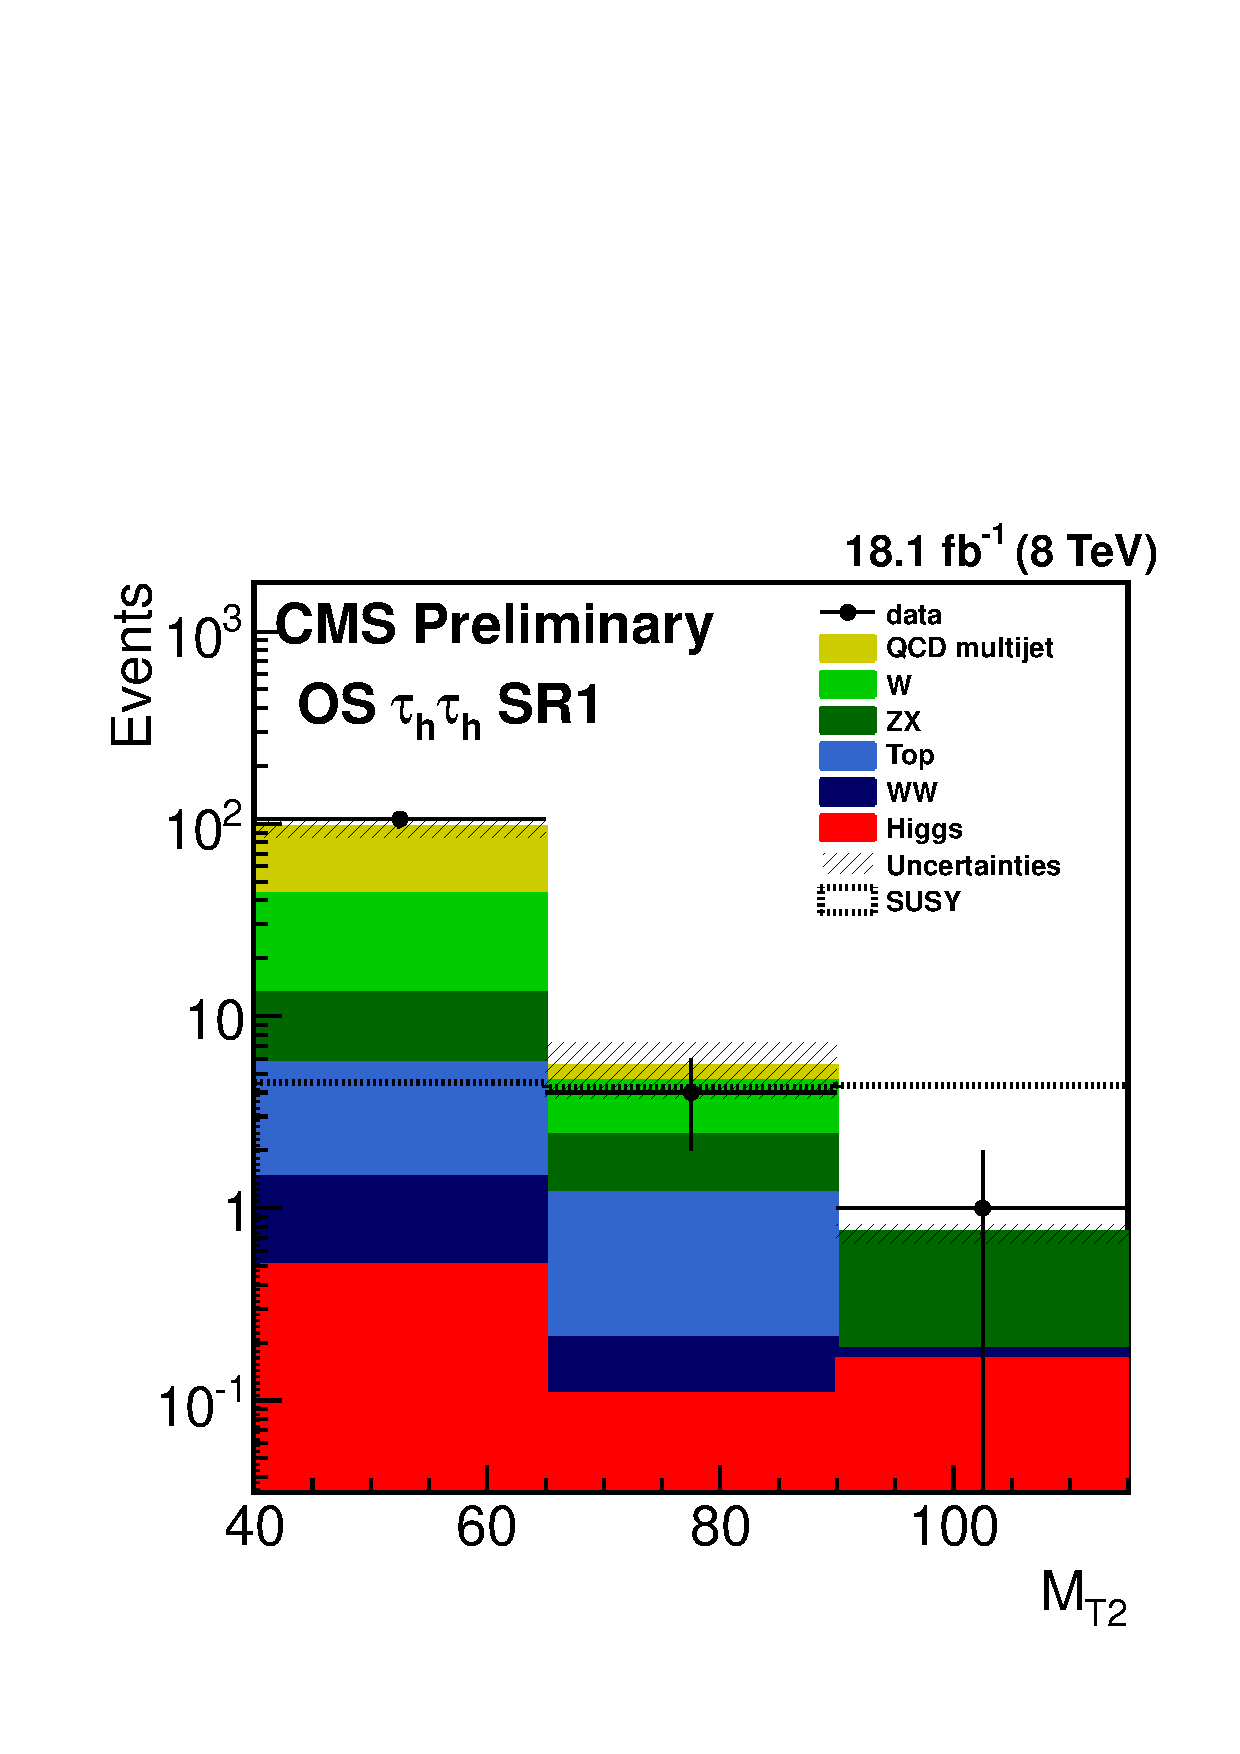
\includegraphics[angle=0,scale=0.375]{TauTauFigs/MT2.pdf}
%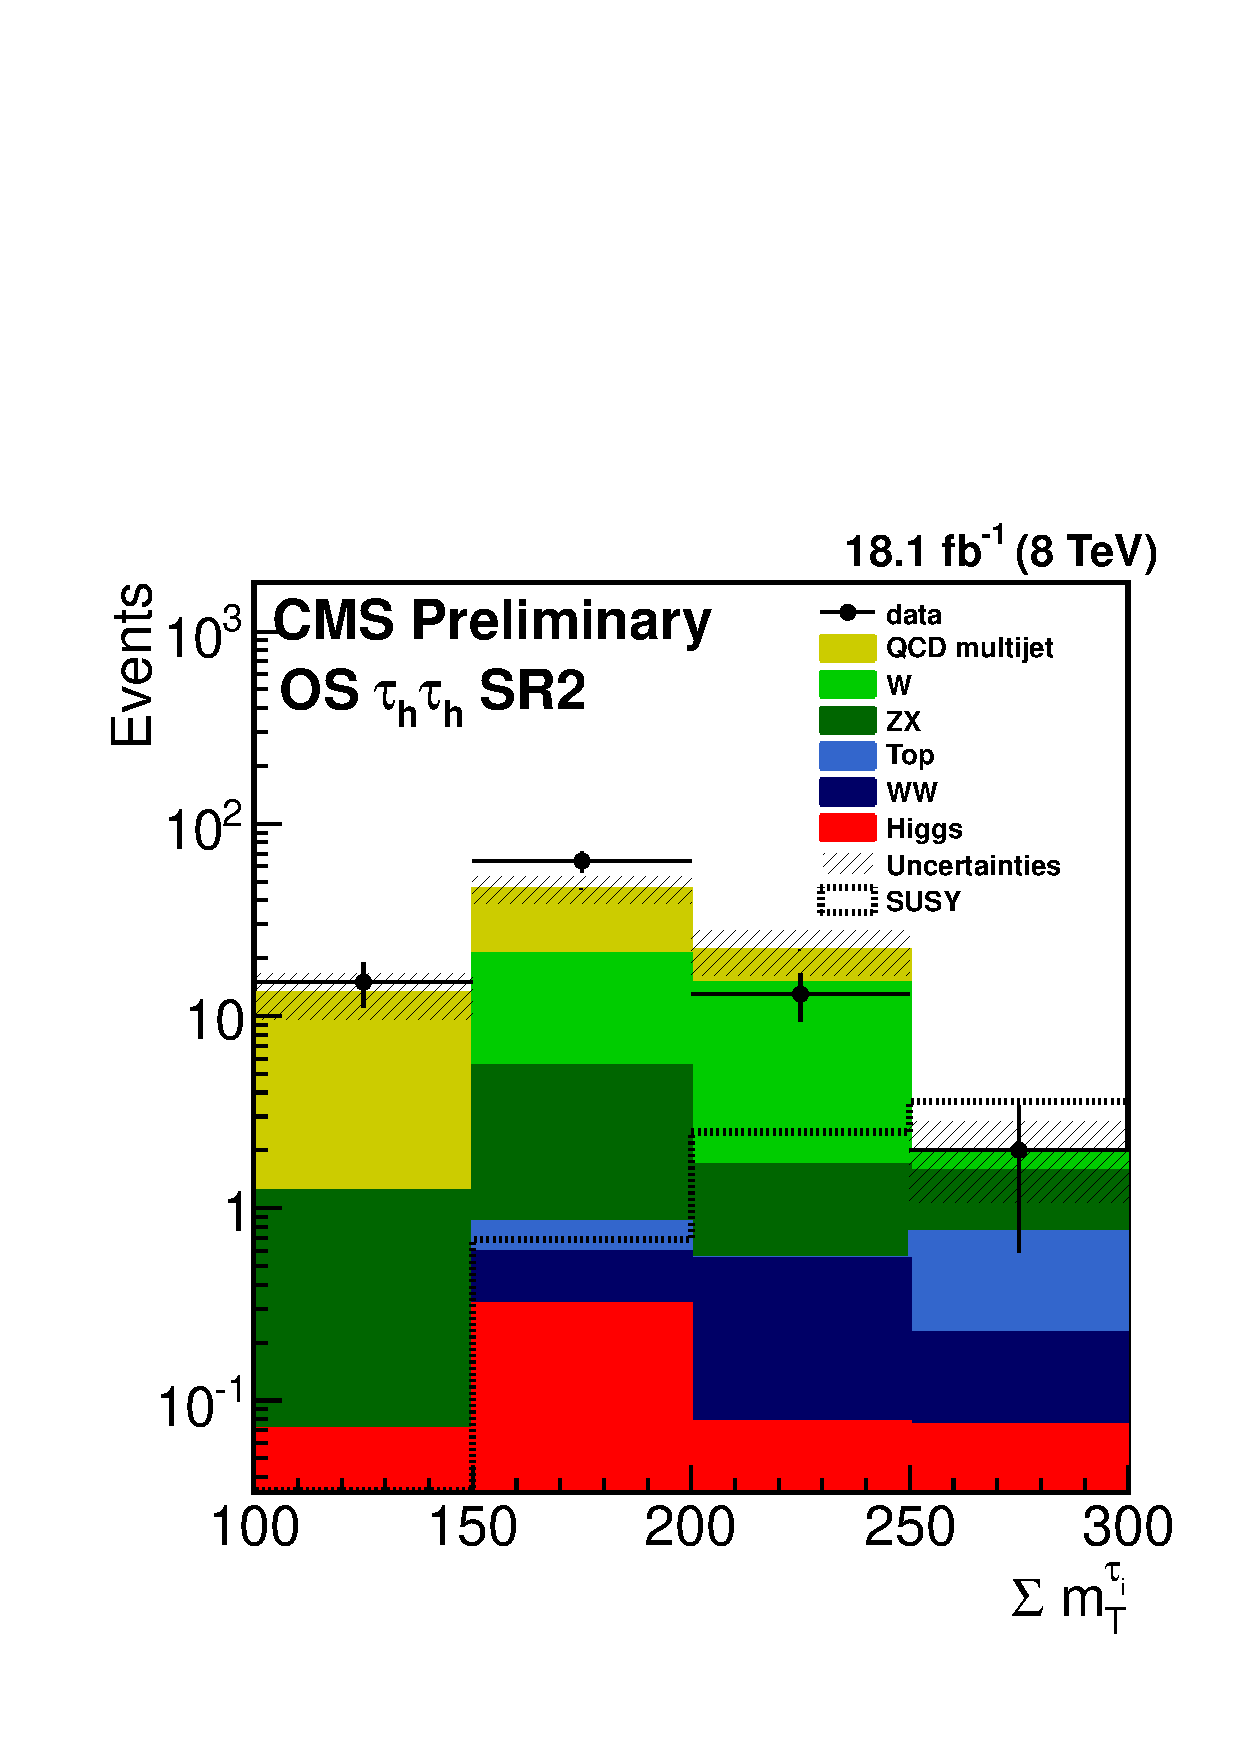
\includegraphics[angle=0,scale=0.375]{TauTauFigs/SumMT.pdf} \\ 
%\caption{The distributions of \mttwo (left) and \SumMT (right) after applying all the selections. 
%The last bins of the histograms correspond to the two signal regions (\binone and \bintwo). The signal distribution is shown for $m_{\chione}=240\GeV,~m_{\PSGczDo}=40\GeV$.}
%\label{fig:comparison}
%\end{figure}
